\documentclass[11pt]{article}
\usepackage[margin=1in]{geometry}
\usepackage{amsmath,amssymb}
\usepackage{booktabs,graphicx,caption}
\usepackage[hidelinks]{hyperref}
\usepackage{natbib}
\newcommand{\e}{\varepsilon}
\setlength{\parskip}{4pt}

\title{Is AI Technical Change Different for the Equilibrium Real Interest Rate?\\
A Flex-Price Ramsey Summary of the First Decade}
\author{Research note (draft)}
\date{October 2026}

\begin{document}
\maketitle

\begin{abstract}
\noindent In a flex-price Ramsey economy, the real interest rate over the first decade of an
AI-driven technology shift is set by one thing: how fast consumption is expected to grow relative to trend.
Three forces change that. \emph{Embodiment} decides whether consumption gains come early or late in the
decade; it is the largest force. \emph{AI versus regular capital} matters mainly through how much
investment AI capital absorbs, and much less through the labor share: even with half of households
hand-to-mouth, the labor-share fall moves the decade-average rate by at most 0.1 percentage points. The
\emph{elasticity of saving} scales every response without changing the ranking:
an intertemporal elasticity of 0.5 or 0.2 multiplies the first-decade effect by about 1.7 or 3.
Habits matter mainly after surprise windfalls. The \emph{level} of adjustment costs matters
more than how they are matched across capital stocks. All shocks are one-time level shifts that raise
long-run output by 10 percent, so the long-run rate is unchanged in this model by construction. Whether AI
changes it depends on saving behavior, which this note holds within Ramsey.
\end{abstract}

\section{The one-line intuition}

With a representative Ricardian household and CRRA preferences ($\theta=1/\text{IES}$), the
Euler equation gives
\begin{gather}
\ln(1+r_{t+1})-\ln(1+r_0)=\theta\,\Delta\ln \tilde c_{t+1},\qquad \tilde c=\frac{c}{Z},\nonumber\\
\sum_{t=0}^{9}\big[\ln(1+r_{t+1})-\ln(1+r_0)\big]=\theta\,\big[\ln\tilde c_{10}-\ln\tilde c_{0}\big].
\label{eq:id}
\end{gather}
The real rate in the first decade is $\theta$ times the expected \emph{catch-up} of consumption
against trend. (The identity is exact without habits; the numerical solutions satisfy it to $10^{-14}$.) The
rate is high when a consumption gain is coming but has not yet arrived. It is low when the gain has already
arrived, or when it is far off. So the questions become: how much of the consumption gain falls inside the
decade, and how much does $\theta$ amplify it?

\paragraph{What is held fixed.}
\begin{itemize}
\item Cobb-Douglas capital-labor bundle, AI capital as a substitute ($\e=1.5$), fixed hours, trend growth 1.5\%,
initial $r=7.5$\%.
\item Equal depreciation for both capital stocks, $d_A=d_K=6.6$\%.
\item Adjustment costs $P_j\tfrac{c_j}{2}(i_j-x_j)^2K_j$, with $c=1/x$ for regular capital (a unit elasticity of
investment to $Q$).
\item Every shock is a permanent level shift in technology, sized for a \emph{10\% long-run output gain}.
Regular-capital progress needs a 29\% improvement and AI progress a 3.4-fold improvement.
\item Two timings. An \emph{S-curve}, $\tfrac12[1-\cos(\pi t/10)]$, is announced at $t=0$ and complete by year 10.
A \emph{jump} is a surprise at $t=0$.
\item The summary statistic is the \emph{decade-average rate}: the mean of $r_1,\dots,r_{10}$ minus 7.5\%, in
percentage points.
\end{itemize}

\section{Results}

\begin{figure}[h]\centering
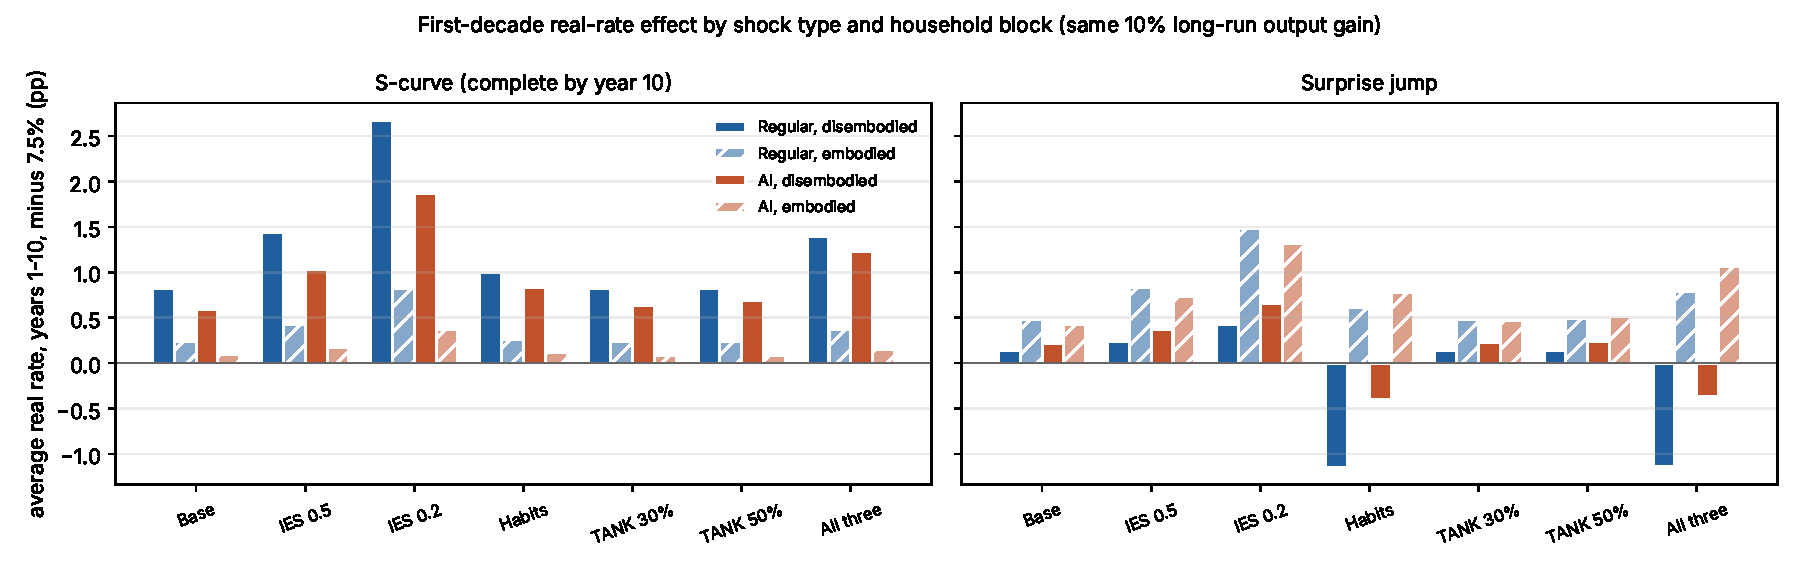
\includegraphics[width=\textwidth]{figures/fig_r_decade.pdf}
\caption{Decade-average real rate relative to 7.5\%, by shock type (solid: disembodied; hatched: embodied; blue: regular capital; orange: AI) and household block.}\label{fig:bars}
\end{figure}

\begin{table}[h]\centering\scriptsize
\caption{Decade-average real rate minus 7.5\% (pp). ``IES'' columns change $\theta$ only. ``Habits'' is $h=0.7$ with $\theta=1$. ``TANK'' is the hand-to-mouth share. ``All three'' is IES 0.5, $h=0.7$ and 30\% hand-to-mouth.}\label{tab:main}
\resizebox{\textwidth}{!}{\begin{tabular}{llccccccc}\toprule
 & & Base & IES 0.5 & IES 0.2 & Habits & TANK 30\% & TANK 50\% & All three\\\midrule
S-curve & Regular, disembodied & +0.83 & +1.44 & +2.67 & +1.00 & +0.83 & +0.83 & +1.40\\
 & Regular, embodied & +0.24 & +0.42 & +0.82 & +0.26 & +0.23 & +0.23 & +0.37\\
 & AI, disembodied & +0.59 & +1.03 & +1.87 & +0.84 & +0.64 & +0.69 & +1.22\\
 & AI, embodied & +0.09 & +0.18 & +0.37 & +0.12 & +0.09 & +0.08 & +0.15\\
\midrule
Jump & Regular, disembodied & +0.13 & +0.23 & +0.42 & -1.14 & +0.13 & +0.13 & -1.14\\
 & Regular, embodied & +0.48 & +0.83 & +1.49 & +0.61 & +0.49 & +0.49 & +0.79\\
 & AI, disembodied & +0.21 & +0.37 & +0.65 & -0.40 & +0.23 & +0.24 & -0.37\\
 & AI, embodied & +0.43 & +0.73 & +1.31 & +0.78 & +0.47 & +0.52 & +1.06\\
\bottomrule\end{tabular}
}
\end{table}

\subsection{Embodiment: when does the consumption gain arrive?}

Take the base column of Table~\ref{tab:main} and the first part of Table~\ref{tab:drivers}.

\begin{table}[h]\centering\scriptsize
\caption{Base household. $\Delta\ln c$ is the gain in detrended consumption from year 0 to 10 (percent); the next column is the right-hand side of (\ref{eq:id}) divided by 10. Wages and output are log deviations (percent) at year 10; labor share in percent.}\label{tab:drivers}
\resizebox{\textwidth}{!}{\begin{tabular}{llccccccc}\toprule
 & & $\Delta\ln c$, yr 0$\to$10 & $\theta\Delta\ln c/10$ & $r_1$ & peak $r$ (yr) & $\ln W$, yr 10 & $\ln Y$, yr 10 & labor share, yr 10\\\midrule
S-curve & Regular, disembodied & 7.7 & +0.77 & 7.69 & 8.75 (5) & 7.7 & 7.6 & 69.7\\
 & Regular, embodied & 2.2 & +0.22 & 7.51 & 7.99 (9) & 2.2 & 1.9 & 69.7\\
 & AI, disembodied & 5.5 & +0.55 & 7.58 & 8.41 (6) & 4.0 & 5.8 & 68.3\\
 & AI, embodied & 0.9 & +0.09 & 7.50 & 7.89 (9) & 1.2 & 1.0 & 69.2\\
\midrule
Jump & Regular, disembodied & 1.3 & +0.13 & 7.67 & 7.67 (0) & 8.3 & 8.2 & 69.7\\
 & Regular, embodied & 4.5 & +0.45 & 8.14 & 8.14 (0) & 4.4 & 4.2 & 69.7\\
 & AI, disembodied & 2.0 & +0.20 & 7.76 & 7.76 (0) & 4.5 & 6.4 & 68.3\\
 & AI, embodied & 4.0 & +0.40 & 8.06 & 8.06 (0) & 2.5 & 3.3 & 68.8\\
\bottomrule\end{tabular}
}
\end{table}

\begin{itemize}
\item \emph{Anticipated shift (S-curve), disembodied.} The technology improves along the S-curve and
consumption follows it, rising 7.7\% (regular) or 5.5\% (AI) over the decade. The rate rises
0.8 and 0.6 points on average and peaks near year 5--6 at 8.8\% and 8.4\%.
\item \emph{Anticipated shift, embodied.} The gain requires building capital first. Investment is front-loaded and
consumption is held down. Consumption gains only 2.2\% (regular) or 0.9\% (AI) by year 10, so the decade-average
rate rises only 0.2 and 0.1 points. (Most of the catch-up falls after year 10.)
\item \emph{Surprise jump, disembodied.} Output and consumption jump at once, so little growth is left to expect
(1.3\% for regular capital): the average is +0.13 points.
\item \emph{Surprise jump, embodied.} Consumption starts low during the investment boom and recovers by 4.5\%:
+0.48 points, with a first-year rate of 8.1\%.
\end{itemize}
The ranking reverses with timing. Disembodied progress raises $r$ most when the shift is anticipated, and embodied
progress raises it most when the shift is a surprise.

\subsection{AI versus regular capital: how much comes from the labor share?}

With the same 10\% output gain, AI progress changes the first-decade rate less than regular-capital progress for an
anticipated shift (0.59 vs 0.83 disembodied; 0.09 vs 0.24 embodied). It changes it a bit more after a disembodied jump (0.21 vs
0.13) and a bit less after an embodied jump (0.43 vs 0.48).

\emph{Why.} AI progress delivers a smaller consumption gain per unit of output gain. Output has to cover
the accumulation of a much larger AI capital stock (3.4-fold technology improvement; capital share rises from 30.4 to
32.2 percent). The wage gain is also smaller, 7.4\% instead of 10\% in the long run (Table~\ref{tab:drivers}), and the
labor share falls by 1.8 points.

\emph{Does the labor share itself matter?} It does not enter the representative-household Euler equation. To test it,
the ``TANK'' columns make 30\% or 50\% of households hand-to-mouth, consuming their wages while Ricardians own all
capital. A falling labor share then lowers hand-to-mouth consumption relative to output, so Ricardian consumption grows
faster and $r$ is higher. The effect is small. For the anticipated disembodied AI shift, the decade-average rate rises
from 0.59 to 0.64 (30\%) or 0.69 (50\%). Regular capital, where the labor share is unchanged, is unaffected, and
embodied AI barely moves. Within a decade, the labor-share fall is too small and too slow to be a main channel
(it is 1.8 points of income in total, and under embodied progress it comes mostly after year 10).

\subsection{Elasticity of saving: how much does the IES amplify?}

\begin{figure}[h]\centering
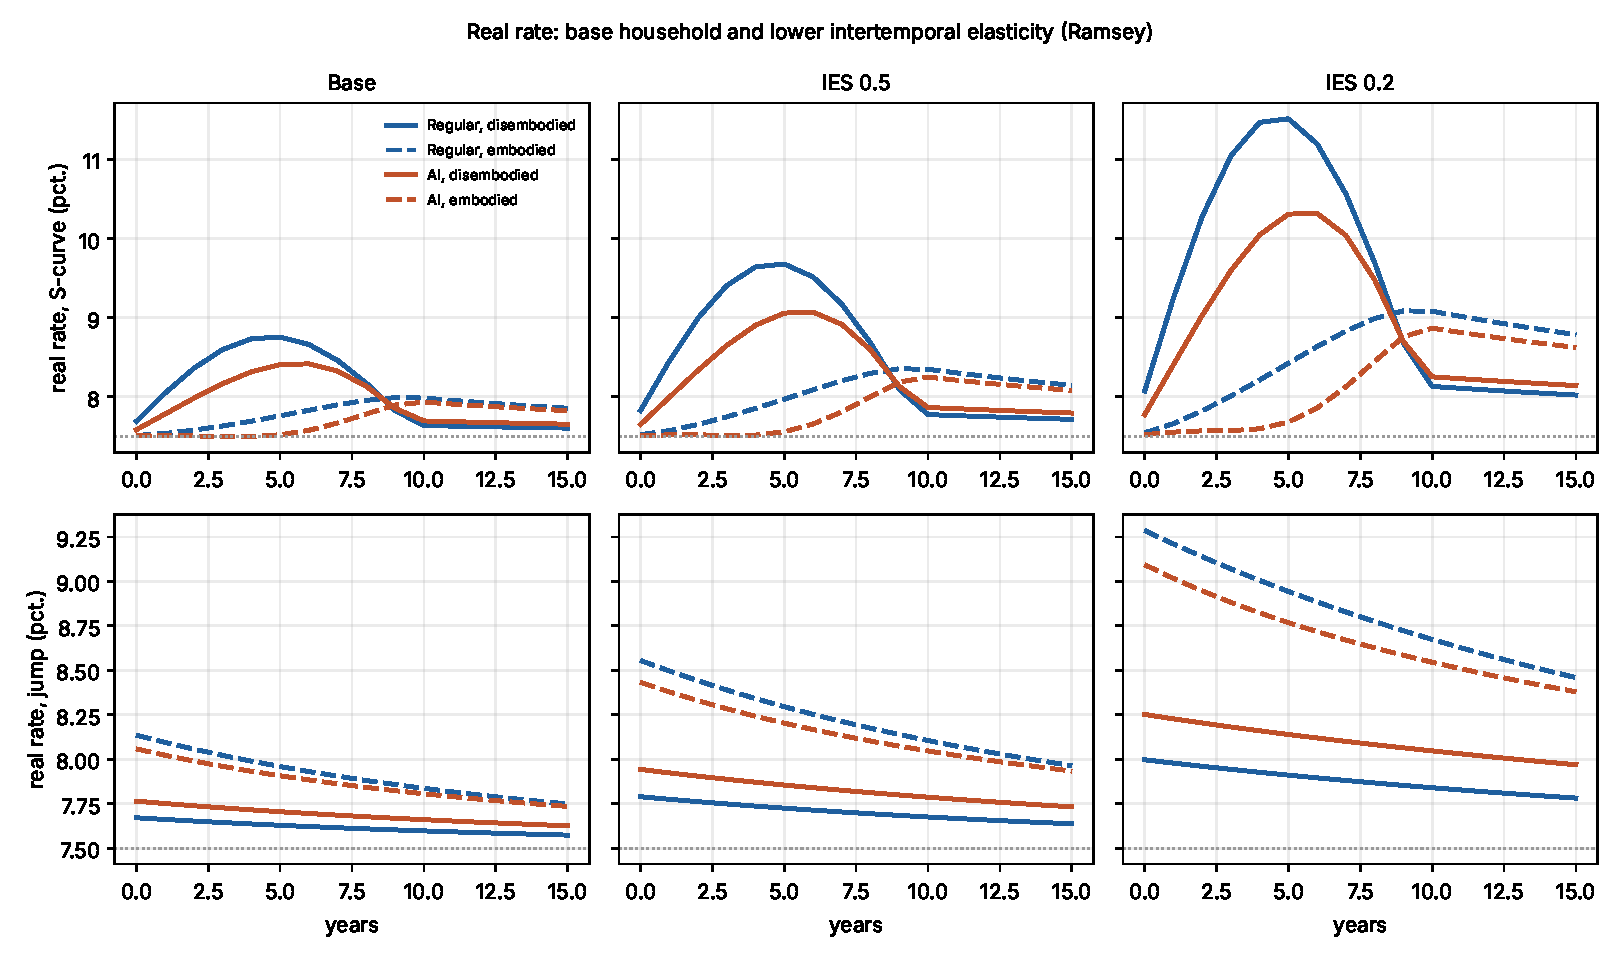
\includegraphics[width=\textwidth]{figures/fig_r_ies.pdf}
\caption{Real-rate paths with $\theta=1,2,5$ (IES 1, 0.5, 0.2).}\label{fig:ies}
\end{figure}

By (\ref{eq:id}), a lower IES multiplies the rate response to a given consumption path by $\theta$. But households also
tilt consumption less, so the consumption catch-up shrinks (for disembodied regular capital, from 7.7\% to 6.7\% and 4.9\%).
The net effect is roughly proportional to $\theta^{0.7}$: the decade-average rate rises by a factor of 1.7 at IES 0.5
and 3.2 at IES 0.2. For the disembodied regular S-curve, the peak rises from 8.75\% to 9.7\% and 11.5\%. The ranking across
embodiment, timing and AI versus regular does not change. A low IES also slows the whole adjustment:
year-10 output gains are smaller (for embodied AI, 1.0\% falls to 0.2\%). So the standard log-utility
baseline probably understates both the size and the persistence of real-rate movements.

\subsection{Habits and hand-to-mouth households}

\begin{figure}[h]\centering
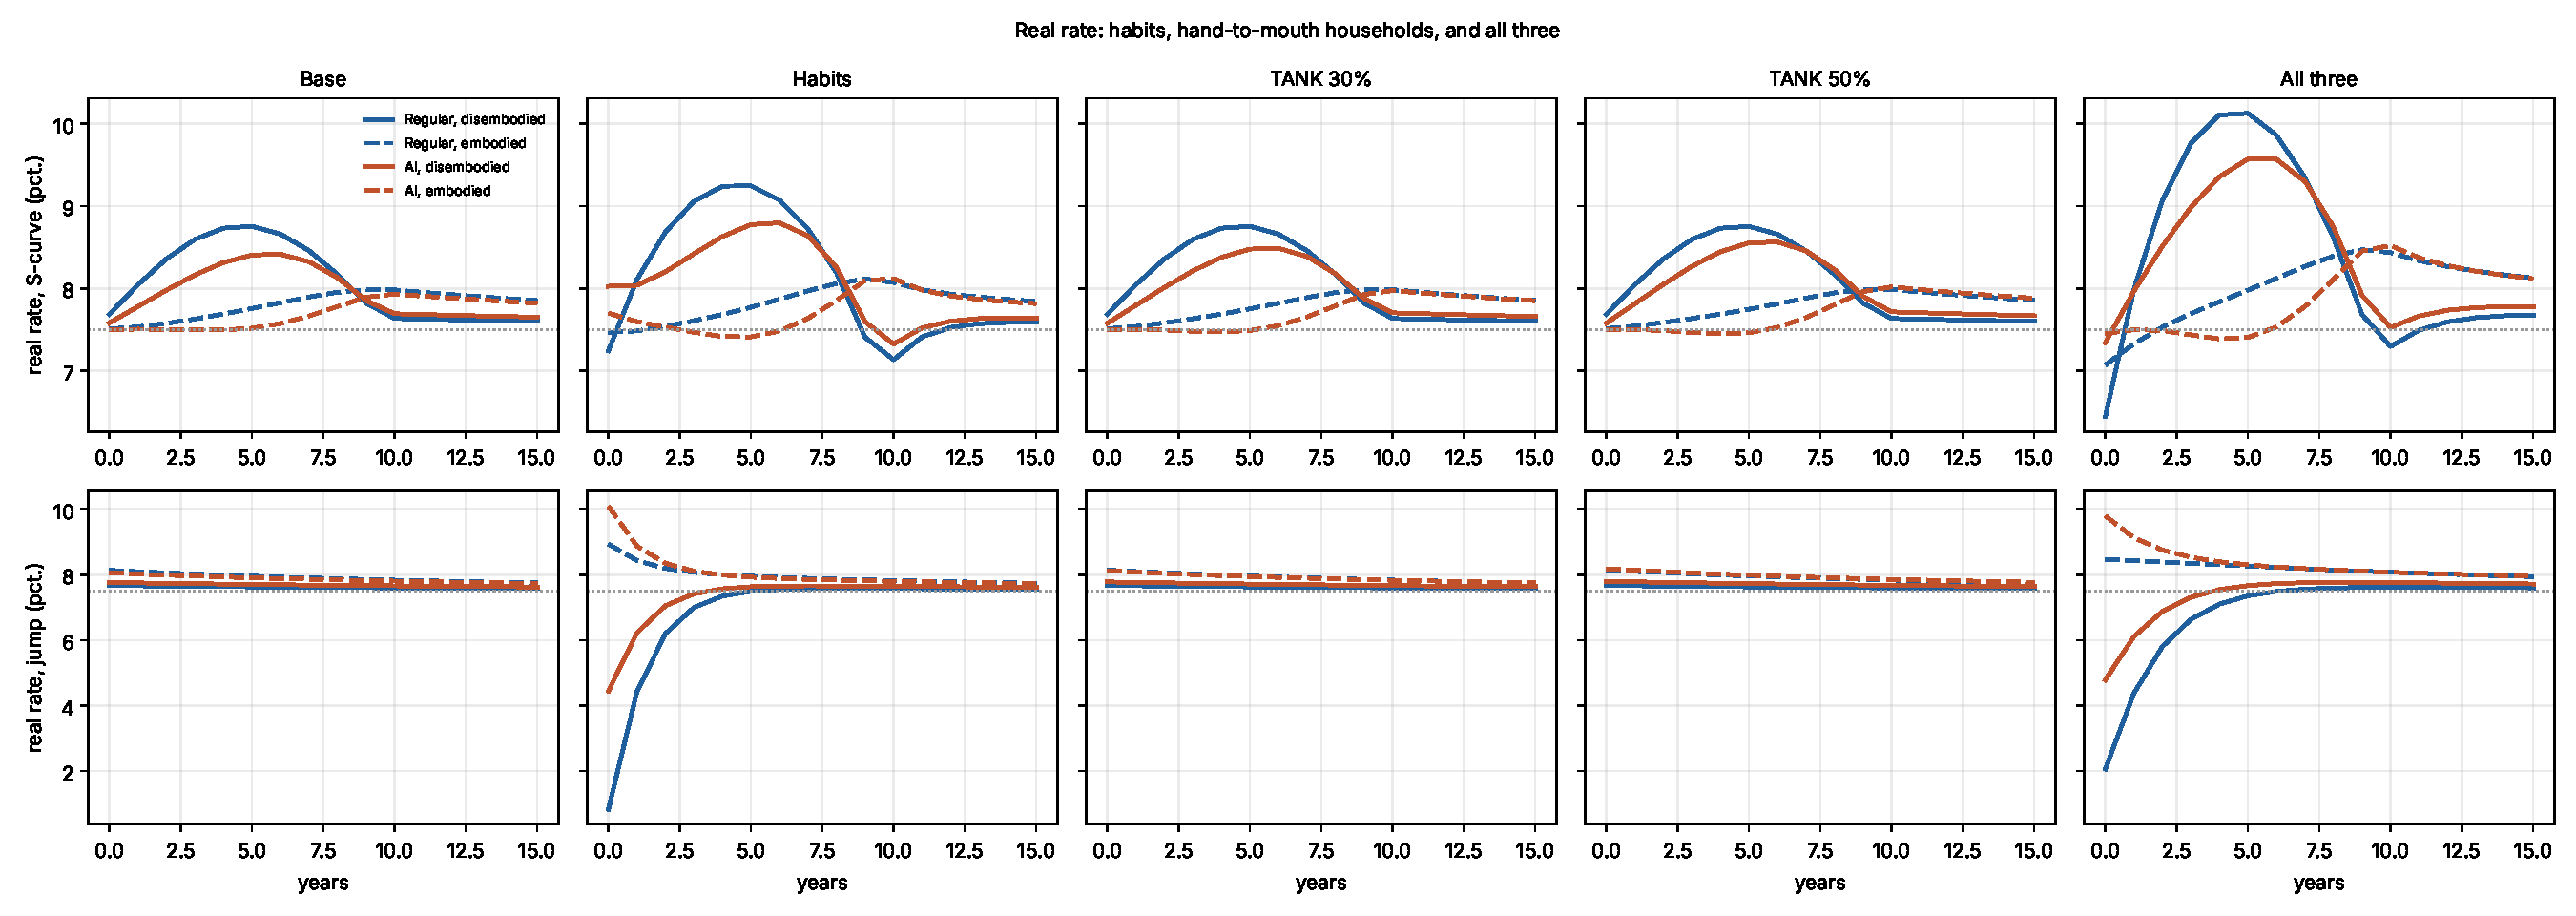
\includegraphics[width=\textwidth]{figures/fig_r_hh.pdf}
\caption{Real-rate paths with habits, hand-to-mouth households, and all three together.}\label{fig:hh}
\end{figure}

\begin{itemize}
\item \emph{Anticipated shifts} are only mildly affected by habits ($h=0.7$ raises the decade average by 0.02--0.25
points), because consumption is already smooth. Their short-run effect is to make the response more hump-shaped.
\item \emph{Surprise disembodied jumps} are strongly affected. The windfall cannot be invested quickly (adjustment costs),
households resist raising consumption (habits), so $r$ must fall to deter saving. The first-year rate falls to 5.2\% at
$h=0.3$ and 0.8\% at $h=0.7$. This is an artifact of a surprise windfall plus costly investment, so I would not rely on it
quantitatively.
\item \emph{Hand-to-mouth households} change very little, as discussed above.
\end{itemize}

\subsection{Calibrating adjustment costs ``similarly''}

Equal depreciation and $c=1/x$ give both capital stocks the same investment response to $Q$ per unit of capital. The
remaining question is whether the two adjust at the same \emph{speed}. I calibrated AI's adjustment cost so that AI capital converges to a
small shock at the same rate as regular capital. The two rates are already close with the same $c$ (5.7\% a year for AI
versus 5.5\% for regular capital), because the curvature of marginal products is similar. The matched $c_A$ is 13.1 against $c_K=12.3$, and
the results match the same-$c$ results to within 0.01 points (Table~\ref{tab:adj}).

\begin{table}[h]\centering\scriptsize
\caption{Decade-average real rate minus 7.5\% (pp) for alternative adjustment-cost calibrations, base household.}\label{tab:adj}
\begin{tabular}{llccccc}\toprule
 & & equal speed & same c & c x 0.5 & c x 2 & none\\\midrule
S-curve & Regular, disembodied & +0.83 & +0.83 & +0.77 & +0.86 & +0.54\\
 & Regular, embodied & +0.24 & +0.24 & +0.09 & +0.33 & -0.55\\
 & AI, disembodied & +0.59 & +0.60 & +0.58 & +0.60 & +0.49\\
 & AI, embodied & +0.09 & +0.09 & +0.05 & +0.11 & -0.14\\
\midrule
Jump & Regular, disembodied & +0.13 & +0.14 & +0.20 & +0.08 & +0.45\\
 & Regular, embodied & +0.48 & +0.48 & +0.69 & +0.31 & +1.48\\
 & AI, disembodied & +0.21 & +0.22 & +0.31 & +0.14 & +0.72\\
 & AI, embodied & +0.43 & +0.44 & +0.55 & +0.32 & +1.09\\
\bottomrule\end{tabular}

\end{table}

What matters is the \emph{level} of $c$, not how it is matched. Without adjustment costs, embodied S-curve
shifts \emph{lower} the first-decade rate ($-0.55$ regular, $-0.14$ AI) because firms wait for cheaper capital. Embodied jumps
raise it more (+1.48, +1.09). Adjustment costs smooth investment, which removes the wait-for-cheaper-capital response. With
no adjustment costs, the AI-versus-regular ranking for an embodied S-curve flips (AI $-0.14$ above regular $-0.55$),
because the dip is deeper for regular capital. With any positive $c$, AI is below regular capital.

\section{Answering the motivating question}

\begin{enumerate}
\item \emph{Is AI technical change different for the equilibrium real interest rate?} In this flex-price Ramsey
benchmark, the first-decade effect is smaller than for regular capital when the shift is anticipated, by about 0.15--0.25 points,
because AI absorbs more of the output gain in accumulation and delivers less consumption growth. After a surprise jump,
the sign depends on embodiment. The difference is modest next to the effect of embodiment, timing and the IES.
\item \emph{Does it depend on the evolution of income shares?} Within the first decade, only weakly. The labor-share fall is
about 1.8 points, mostly after year 10 for embodied progress, and it moves the decade-average rate by at most 0.1
points even with half the population hand-to-mouth. In the long run, income shares do not move $r$ in Ramsey at all,
because the Euler equation pins it. The earlier comparison with Solow, Diamond and annual-OLG saving shows that the
income-share channel would matter for long-run $r$ only if saving is less elastic than Ramsey implies.
\item \emph{What would be needed to make shares matter?} Saving that depends on the type of income, and a
labor-share fall that is large and early.
\end{enumerate}

\paragraph{Caveats.} Hours are fixed. All shocks are level shifts sized for the same long-run output gain, not shocks of equal
technical size. The habit specification is additive and internal, with a strong annual $h$. The adjustment-cost level is
unobserved, and Table~\ref{tab:adj} shows it is the most important calibration choice here for embodied progress.
Nominal rigidities, the next step, would turn the response of $r$ to consumption growth into a response of output as well.

\appendix
\section{Verification}
All results come from \texttt{ramsey\_variants.py} (built on \texttt{capital\_cases.py}). Every transition is a nonlinear
perfect-foresight solve of the full equilibrium. The model uses the Euler equations of both capital stocks with
the household block above, 250 years, with residuals below $10^{-10}$. The pre-shock balanced growth path satisfies
the Euler equations for every household block. For $h=0$, (\ref{eq:id}) holds to $10^{-14}$, and every shock reaches the 10 percent output gain to within $10^{-4}$ (the slowest case is IES 0.2).

\begin{table}[h]\centering\scriptsize
\begin{tabular}{lc}\toprule Check & max abs. error\\\midrule
residual & 7.7e-11\\
long-run ln Y = 10\% & 8.6e-05\\
identity sum ln(1+r) = theta dln c & 1.3e-15\\
BGP satisfies the Euler equations & 5.5e-14\\
\bottomrule\end{tabular}

\end{table}

\end{document}
